\subsection{RQ2: Is there a tolerance limit for ESP?}\label{sect:rq2}

\begin{figure}[!t]
\begin{lstlisting}
_  = None;  Coc2tunings = [[
#              vlow  low   nom   high  vhigh  xhigh   
# scale factors:
'Flex',        5.07, 4.05, 3.04, 2.03, 1.01,     _],[
'Pmat',        7.80, 6.24, 4.68, 3.12, 1.56,     _],[
'Prec',        6.20, 4.96, 3.72, 2.48, 1.24,     _],[
'Resl',        7.07, 5.65, 4.24, 2.83, 1.41,     _],[
'Team',        5.48, 4.38, 3.29, 2.19, 1.01,     _],[
# effort multipliers:        
'acap',        1.42, 1.19, 1.00, 0.85, 0.71,    _],[
'aexp',        1.22, 1.10, 1.00, 0.88, 0.81,    _],[
'cplx',        0.73, 0.87, 1.00, 1.17, 1.34, 1.74],[
'data',           _, 0.90, 1.00, 1.14, 1.28,    _],[
'docu',        0.81, 0.91, 1.00, 1.11, 1.23,    _],[
'ltex',        1.20, 1.09, 1.00, 0.91, 0.84,    _],[
'pcap',        1.34, 1.15, 1.00, 0.88, 0.76,    _],[ 
'pcon',        1.29, 1.12, 1.00, 0.90, 0.81,    _],[
'plex',        1.19, 1.09, 1.00, 0.91, 0.85,    _],[ 
'pvol',           _, 0.87, 1.00, 1.15, 1.30,    _],[
'rely',        0.82, 0.92, 1.00, 1.10, 1.26,    _],[
'ruse',           _, 0.95, 1.00, 1.07, 1.15, 1.24],[
'sced',        1.43, 1.14, 1.00, 1.00, 1.00,    _],[ 
'site',        1.22, 1.09, 1.00, 0.93, 0.86, 0.80],[ 
'stor',           _,    _, 1.00, 1.05, 1.17, 1.46],[
'time',           _,    _, 1.00, 1.11, 1.29, 1.63],[
'tool',        1.17, 1.09, 1.00, 0.90, 0.78,    _]]

def COCOMO2(project,  a = 2.94, b = 0.91, # defaults
                      tunes= Coc2tunings):# defaults 
  sfs ems, kloc  = 0,1,22          
  scaleFactors, effortMultipliers = 5, 17
  for i in range(scaleFactors):
    sfs += tunes[i][project[i]]
  for i in range(effortMultipliers):
    j = i + scaleFactors
    ems *= tunes[j][project[j]] 
  return a * ems * project[kloc] ** (b + 0.01*sfs) 
\end{lstlisting}
\caption{COCOMO-II: effort estimates from a {\em project}.
Here, {\em project} has up to 24 attributes  (5 scale
factors plus 17 effort multipliers plus KLOC plus. in the training data, the actual effort).
Each attribute except KLOC and effort is scored
using the scale very low = 1, low=2, etc.
For an explanation of the attributes shown in
green, see \fig{cparems}.}\label{fig:coc2}
\end{figure}



To conduct the perturbation study for identifying a point of tolerance,  we use  COCOMO since its internal details have been fully published~\cite{boehm00b}. Also, we can access a full implementation of the  2000 COCOMO model. Further, we have access to four interesting  COCOMO data sets. With one exception, our learning experiments do not use the data that generated   standard COCOMO. That exception is the  COC81 data-- which  lets us  compare new methods against the  labor intensive methods used to make standard COCOMO-- see \fig{dataused}.

The primary method used in our study is the COCOMO2 which is described using simple python code in \fig{coc2}. The impact of noise in \textit{KLOC} is studied by varying $\mathit{KLOC}$ as follows

\begin{equation}
    \label{eq:kloc}
    \mathit{KLOC} = \mathit{KLOC}*((1- n) + (2*n*r))
\end{equation}

where $n \in [0.2, 0.4, 0.6, 0.8, 1.0]$ is the level of noise we are exploring and $r$ is a random number
$0 \le r \le 1$. In the results, any result
prefixed with {\em 0.2} to {\em 1.0} shows what happens
when the KLOCs were varied by 20\% to 100\% respectively.

\begin{figure*}[!ht]
    \centering
    \begin{minipage}[c]{\linewidth}
    \begin{mdframed}
    Scott-Knott procedure recommended by Mittas \& Angelis in their 2013 IEEE TSE paper~\cite{mittas13}.  This method sorts a list of $l$ treatments with $ls$ measurements by their median score. It then splits $l$ into sub-lists $m,n$ in order to maximize the expected value of differences  in the observed performances before and after divisions. E.g. for lists $l,m,n$ of size $ls,ms,ns$ where $l=m\cup n$:
     \[E(\Delta)=\frac{ms}{ls}abs(m.\mu - l.\mu)^2 + \frac{ns}{ls}abs(n.\mu - l.\mu)^2\]

    Scott-Knott then applies some statistical hypothesis test $H$ to check if $m,n$ are significantly different. If so, Scott-Knott then recurses on each division.Scott-Knott is better than an all-pairs hypothesis test of all methods; e.g. six treatments can be compared \mbox{$(6^2-6)/2=15$} ways.  A 95\% confidence test run for each comparison has  a very low total confidence: \mbox{$0.95^{15} = 46$}\%. To avoid an all-pairs comparison, Scott-Knott only calls on hypothesis tests {\em after} it has found splits that maximize the performance differences.

    For this study, our hypothesis test $H$ was a conjunction of the A12 effect size test(endorsed by Arcuri \etal in ICSE '11 \cite{arcuri11}) of  and non-parametric bootstrap sampling \cite{efron93}; i.e. our Scott-Knott divided the data if {\em both}
    bootstrapping and an effect size test agreed that the division was statistically significant (99\% confidence) and not a ``small'' effect ($A12 \ge 0.6$). 
    For a justification of the use of non-parametric
    bootstrapping, see Efron \&
    Tibshirani~\cite[p220-223]{efron93}.
    For a justification of the use of effect size tests
    see Shepperd \& MacDonell~\cite{shepperd12a}; Kampenes~\cite{kampenes07}; and
    Kocaguneli et al.~\cite{kocharm13}. These researchers
    warn that even if an
    hypothesis test declares two populations to be
    ``significantly'' different, then that result is
    misleading if the ``effect size'' is very small.
    Hence, to assess 
    the performance differences 
    we first must rule out small effects.
    Vargha and Delaney's
    non-parametric 
    A12 effect size test 
    explores
    two lists $M$ and $N$ of size $m$ and $n$:
    \[A12 = \left(\sum_{x\in M, y \in N} 
    \begin{cases} 
    1   & \mathit{if}\; x > y\\
    0.5 & \mathit{if}\; x == y
    \end{cases}\right) / (mn)
    \]
    This expression computes the probability that numbers in one sample are bigger than in another.
    This test was recently 
    endorsed by Arcuri and Briand
    at ICSE'11~\cite{arcuri11}.
    \end{mdframed}
    \caption{Scott-Knott Test}
    \end{minipage}
    \label{fig:sk}
\end{figure*}

% Please add the following required packages to your document preamble:
% \usepackage{multirow}
\begin{figure}[!t]
\begin{center}
\caption{NASA10}
\scriptsize
\label{fig:nasa10}
\begin{tabular}{|r|c|c|c|c|}
\hline
\multicolumn{1}{|c|}{\multirow{2}{*}{\textbf{Name}}} & \multicolumn{2}{c|}{\textbf{Med}}     & \multicolumn{2}{c|}{\textbf{IQR}} \\ \cline{2-5} 
\multicolumn{1}{|c|}{}                               & \textbf{Rank} & \textbf{Med $\pm$ IQR} & \textbf{Rank} & \textbf{Med $\pm$ IQR} \\ \hline
    COCOMO2  & 1 & 43 $\pm$ 48   & 1    & 1 $\pm$ 1     \\ \cline{4-5}
20\%:COCOMO2 & 1 & 41 $\pm$ 57   & 2    & 13 $\pm$ 19   \\ \cline{4-5}
40\%:COCOMO2 & 1 & 41 $\pm$ 50   & 3    & 28 $\pm$ 14   \\ \cline{2-3}
60\%:COCOMO2 & 2 & 46 $\pm$ 54   & 3    & 34 $\pm$ 44   \\ 
80\%:COCOMO2 & 2 & 50 $\pm$ 54   & 3    & 44 $\pm$ 39   \\
100\%:COCOMO2 & 2 & 68 $\pm$ 59  & 3    & 49 $\pm$ 32    \\ \hline         
\end{tabular}


\caption{COC05}
\scriptsize
\label{fig:coc05}
\begin{tabular}{|r|c|c|c|c|}
\hline
\multicolumn{1}{|c|}{\multirow{2}{*}{\textbf{Name}}} & \multicolumn{2}{c|}{\textbf{Med}}     & \multicolumn{2}{c|}{\textbf{IQR}} \\ \cline{2-5} 
\multicolumn{1}{|c|}{}                               & \textbf{Rank} & \textbf{Med $\pm$ IQR} & \textbf{Rank} & \textbf{Med $\pm$ IQR} \\ \hline
    COCOMO2  & 1 & 13 $\pm$ 53   & 1    & 1 $\pm$ 1     \\ \cline{4-5}
20\%:COCOMO2 & 1 & 14 $\pm$ 53   & 2    & 8 $\pm$ 22   \\ 
40\%:COCOMO2 & 1 & 19 $\pm$ 50   & 2    & 14 $\pm$ 42   \\ \cline{2-5}
60\%:COCOMO2 & 2 & 24 $\pm$ 57   & 3    & 25 $\pm$ 67   \\ 
80\%:COCOMO2 & 2 & 25 $\pm$ 46   & 3    & 25 $\pm$ 79   \\
100\%:COCOMO2 & 2 & 26 $\pm$ 71  & 3    & 30 $\pm$ 96    \\ \hline    
\end{tabular}

\caption{NASA93}
\scriptsize
\label{fig:nasa93}
\begin{tabular}{|r|c|c|c|c|}
\hline
\multicolumn{1}{|c|}{\multirow{2}{*}{\textbf{Name}}} & \multicolumn{2}{c|}{\textbf{Med}}     & \multicolumn{2}{c|}{\textbf{IQR}} \\ \cline{2-5} 
\multicolumn{1}{|c|}{}                               & \textbf{Rank} & \textbf{Med $\pm$ IQR} & \textbf{Rank} & \textbf{Med $\pm$ IQR} \\ \hline
    COCOMO2  & 1 & 14 $\pm$ 39   & 1    & 1 $\pm$ 2     \\ \cline{4-5}
20\%:COCOMO2 & 1 & 14 $\pm$ 40   & 2    & 5 $\pm$ 8   \\ \cline{4-5}
40\%:COCOMO2 & 1 & 15 $\pm$ 43   & 3    & 8 $\pm$ 14   \\ \cline{4-5}
60\%:COCOMO2 & 1 & 16 $\pm$ 44   & 4    & 12 $\pm$ 24   \\ \cline{2-3}
80\%:COCOMO2 & 2 & 20 $\pm$ 40   & 4    & 13 $\pm$ 28   \\\cline{4-5}
100\%:COCOMO2 & 2 & 27 $\pm$ 42  & 5    & 19 $\pm$ 36    \\ \hline  
\end{tabular}

\caption{COC81}
\scriptsize
\label{fig:coc81}
\begin{tabular}{|r|c|c|c|c|}
\hline
\multicolumn{1}{|c|}{\multirow{2}{*}{\textbf{Name}}} & \multicolumn{2}{c|}{\textbf{Med}}     & \multicolumn{2}{c|}{\textbf{IQR}} \\ \cline{2-5} 
\multicolumn{1}{|c|}{}                               & \textbf{Rank} & \textbf{Med $\pm$ IQR} & \textbf{Rank} & \textbf{Med $\pm$ IQR} \\ \hline
    COCOMO2  & 1 & 3 $\pm$ 18   & 1    & 0 $\pm$ 1     \\ \cline{4-5}
20\%:COCOMO2 & 1 & 4 $\pm$ 20   & 2    & 2 $\pm$ 4   \\ \cline{4-5}
40\%:COCOMO2 & 1 & 4 $\pm$ 16   & 3    & 4 $\pm$ 7   \\ \cline{2-5}
60\%:COCOMO2 & 2 & 6 $\pm$ 19   & 4    & 6 $\pm$ 11   \\ \cline{4-5}
80\%:COCOMO2 & 2 & 6 $\pm$ 21   & 5    & 7 $\pm$ 15   \\
100\%:COCOMO2 & 2 & 8 $\pm$ 18  & 5    & 8 $\pm$ 18    \\ \hline        
\end{tabular}
\end{center}
\end{figure}

\begin{figure}
    \centering
    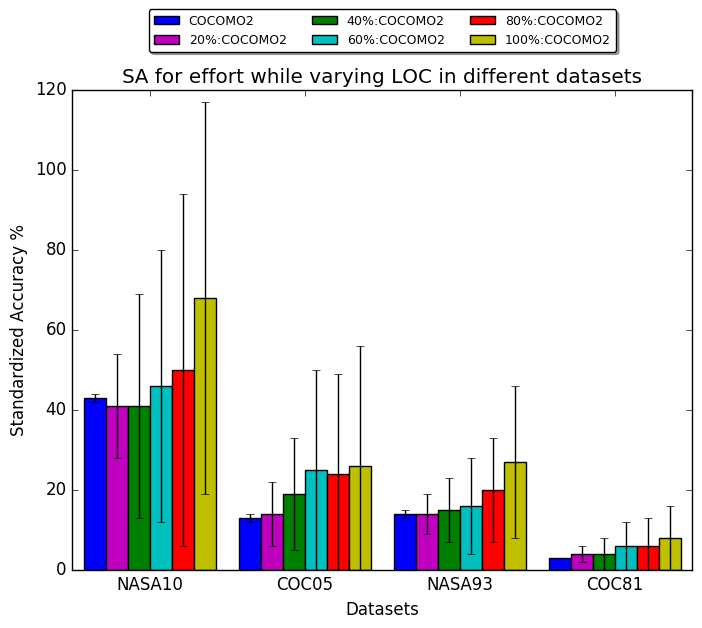
\includegraphics[scale=0.45]{Figs/sa.png}
    \caption{Standarized Accuracy for effort while varying LOC in different datasets.}
    \label{fig:sa_datasets}
\end{figure}

% \begin{equation}\label{eq:mre}
% \mbox{$ \mathit{MRE}=\frac{abs(\mathit{actual} - \mathit{predicted})}{\mathit{actual}}$}
% \end{equation}

\begin{equation}\label{eq:sa}
\mbox{$ \mathit{SA}=\frac{abs(\mathit{actual} - \mathit{predicted})}{\mathit{\sum_{i=1}^{1000}|\pmb{choice}(all) - predicted|}/1000}$}
\end{equation}

Each of the four tables(\fig{nasa10}, \fig{coc05}, \fig{nasa93} \& \fig{coc81}) represent Standardized Accuracy(SA) values seen in leave-one-out-studies, repeated twenty times for the dataset highlighted in table\'s title. i.e. For every project in a dataset, the value of $r$ from \eq{kloc} is changed 20 times and KLOC is estimated and then substituted in \eq{one}. SA proposed by Shepperd and MacDonell~\cite{shepperd12a} is calculated as shown in \eq{sa} where $actual$ is the true value of effort, $predicted$ is the estimated value, $all$(array) is all the effort values in the dataset and $\pmb{choice}$ randomly picks one value from an array.  The first column in each table denotes the name of the method. COCOMO2 represents estimating effort using COCOMO-II as shown in \fig{coc2}. $x$\%:COCOMO2 represents COCOMO-II where KLOC is perturbed with an error of $x$\% using \eq{kloc}. Column 3 highlights the median and IQR for the median of the SA while column 5 highlights the median and IQR of the IQR of SA.  {\em Better} methods appear {\em higher} in the tables.In these tables, median and IQR are the 50th and the  (75-25)th percentiles. Horizontal lines divide the ``ranks'' found by our Scott-Knott+bootstrapping+effect size tests (shown in column ``Rank''). In these tables we can observe that upto 40\% error in $KLOC$ is tolerable and error greater than that significantly changes the estimate. This observation is further backed by \fig{sa_datasets} which graphically show how the SA changes as we increase the error for the 4 datasets. Thus, there is point of tolerance beyond which estimation error increases significantly.